% file to contain information on examples
%==============================================================================
\chapter{Examples Explained - WIP}
Examples are located in the \verb|0-examples| folder and are designed to be run in batch mode.
This means that each example copies any required system, model, or modulation file to the main PST directory before running.
Typically, each example folder contains a \verb|.m| file that starts with \verb|run| that can be used to run the example.
As example cases are located on a github repository, relative file paths are used so that examples can be run without much difficulty from various different machines.
While most examples can be run in multiple versions of PST, some functionality can only be found in specific versions.

\noindent The general structure of created examples tend to reflect the following:
\begin{enumerate}
\itemsep 0em
\item Clear all variables, close all figures, and clear the command window
\item Define which version of PST to use
\item Create a relative path to the root directory of chosen PST version
\item Copy any system, model, or modulation file to the PST root directory
\item Run \verb|s_simu|
\item Save output data
\item Restore any model, or modulation file to original state
\item Create data plots
\end{enumerate}

%=================================================================
\pagebreak
\section{Standard Faulting (hiskens)}
Standard PST simulations involve some kind of fault defined in the \verb|sw_con| array.
This example (located in the \verb|hiskens| folder) is included to showcase some simple differences between PST versions using a standard test case.
System data for this example comes from a report by Ian Hiskens \cite{hiskens2013} which summarized a study of an IEEE 10 generator, 39 bus system.
Ryan Elliott at Sandia National Labs recreated the system in a PST format and provided the data file for this project.
A one-line diagram of the system is shown in Figure \ref{fig: hiskens oneline}.

\begin{figure}[H]
	\centering
	\footnotesize
	\includegraphics[width=.85\linewidth]{figures/hiskens/hiskensOneline}
	\caption{IEEE 39 bus network.}
	\label{fig: hiskens oneline}
\end{figure}%\vspace{-1 em}

The simulated event was a 0.1 second three-phase fault with no loss of line between bus 2 and 3.
The \verb|run_datane_hiskens.m| file can be used to run the simulation.
Figure \ref{fig: hiskens results} shows the resulting fault bus voltage magnitude and system generator speeds.

\begin{figure}[H]
	\centering
	\footnotesize
	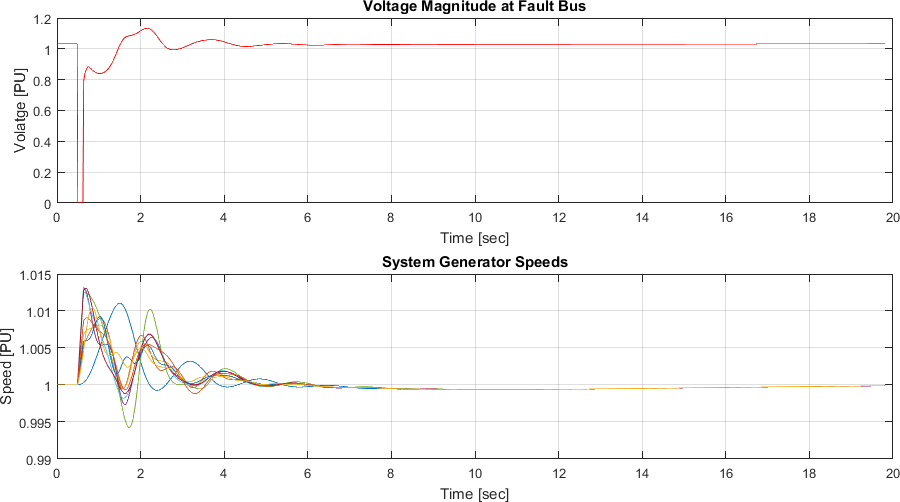
\includegraphics[width=\linewidth]{figures/hiskens/hiskensResults}
	\caption{Hiskens Example Fault Bus Voltage and Generator Speeds.}
	\label{fig: hiskens results}
\end{figure}%\vspace{-1 em}

All PST versions (when using the same models) provide the same results, but there are differences in simulation speed and data output.
Table \ref{tab: hiskens} shows that the PST 4 simulation was roughly twice as fast as PST version 2 or 3, saved less data, and left fewer variables in the MATLAB workspace post simulation.
These improvements are likely due to the restructuring of global variables and code to remove any `all zero` data from being saved.\\

% table data for hiskens fault comparison 


\begin{table}[H]
%\resizebox{\linewidth}{!}{ % Use to resize large tables
\singlespacing
	\begin{tabular}{@{} L{1.75cm} 
	R{2cm} R{2cm}  R{2cm} @{}} 	
		\toprule % @ signs to remove extra L R space
		\footnotesize % this will affect the table font (makse it 10pt)
		\raggedright % for non justified table text
						
										
										
		PST Version	&	Simulation Time [seconds]	&	Resulting Workspace Variables	&	Saved Data Size [KB]	\\ \midrule	
		2.3	&	16.56	&	206	&	7,549	\\	
		3.1	&	16.70	&	210	&	7,548	\\	
		SETO	&	8.42	&	24	&	3,965	\\	
		4	&	7.96	&	6	&	3,974	\\	\bottomrule

													
	\end{tabular}

	\caption{PST Version Comparisons of Hiskens Example.}
	\label{tab: hiskens}
%	}%end resize box
\end{table}

\pagebreak
\begin{itemize}
\item Experimental VTS
\item AGC
\item AGC interchange modulation
\item Extended term with VTS
\item MiniWECC via Dan
\item Experimental Un-tripping
\item Modulation via \verb|_mod| files
\item Linear simulation where applicable...
\item Combine examples? 
\end{itemize}

Variables to note in associated examples (where \verb|x| is the internal model number):
\begin{itemize}
\item exciter $V_{ref} = $ \verb|g.exc.exc_pot(x,3)|
\item governor $P_{ref} = $ \verb|g.tg.tg_pot(x,5)|
\item governor $\omega_{ref} = $ \verb|g.tg.tg_con(x,3)|
\end{itemize}

\pagebreak
\section{Automatic Generation Control (AGC)} 
A variety of examples were created for AGC testing.
While some may use VTS, this section covers information only related to AGC.
The VTS example section contains VTS specific information.

The \verb|0-examples/AGC| folder contains all system and modulation files associated with the AGC examples.
The \verb|run***| files are designed to run PST in using the batch mode.
\section{Variable Time Step - WIP}
